%=========================================================

% Here you can choose to compile with or without solutions.
% However, this definition is ignored if you use any
% command from the `Makefile`.
\providecommand{\withSol}{\iftrue}

%=========================================================

\documentclass
[twoside,english,colorbacktitle,accentcolor=tud9c]
{tudexercise}

\usepackage[T1]{fontenc}
\usepackage[latin9]{inputenc}
\usepackage{amstext}
\usepackage{amsmath}
\usepackage{graphicx}
\usepackage{setspace}
\usepackage{multicol}
\usepackage{mathtools}
\usepackage{dsfont}
\usepackage{units}
\usepackage{subfigure}
\usepackage{color}
\usepackage{booktabs}
\usepackage{fancyref}
\usepackage[ngerman,english]{babel}
\usepackage{commath}
\usepackage{listings}

%=========================================================

\def\homework{1}
\def\homeworkVer{1}
\def\homeworkSolVer{1}
\def\lecture{Machine Learning}
\def\semester{Summer Semester 2019}
\def\prof{Prof. Dr. J. Peters, H. Abdulsamad, S. Stark, D.Koert}
\def\deadline{Due date: Sunday, 26 May 2019 (before midnight)\\
Hand in a PDF over Moodle \textbf{and} a printed version to the postbox at (S2/02 | E315)}

%=========================================================

\ifcsname withSol\endcsname\else
  \expandafter\let\csname withSol\expandafter\endcsname
                  \csname iffalse\endcsname
\fi

\withSol
	\usepackage[solutions]{iasHomework}
\else
	\usepackage{iasHomework}
\fi

%=========================================================

% USE YOUR NAMES!
\newcommand{\studentdata}{Peter Nickl, 1941346 \qquad Steffen Schäfer, 111111}
%\newcommand{\studentdata}{John Doe, 1234567 \qquad Jane Doe, 7654321}

\begin{document}
	
	\hwtitle{}
	\maketitle
	
	\begin{examheader}
		\normalsize
		\vspace{-1em}
		Name, Surname, ID Number \hfill \studentdata{}
		\vspace{-1em}
	\end{examheader} 
	
	\textbf{Name, Surname, ID Number \hfill \studentdata{}}

	\newif\ifvimbug
\vimbugfalse

\ifvimbug
\begin{document}
\fi

\exercise{Linear Algebra Refresher}
 

\begin{questions}

%----------------------------------------------

\begin{question}{Matrix Properties}{5}
A colleague of yours suggests matrix addition and multiplication are similar to scalars, thus commutative, distributive and associative properties can be applied.
Prove if matrix addition and multiplication are commutative and associative analytically or give counterexamples. 
Is matrix multiplication distributive with respect to matrix addition? 
Again, prove it analytically or give a counterexample.
Considering three matrices $ A, B, C$ of size $n\times n$.

\begin{answer}
To answer the questions examples calculated by following matrices will be used:


\[
A=
\begin{bmatrix}
2 & -1  \\
0 &  1 
\end{bmatrix}\quad
B=
\begin{bmatrix}
1 & 0  \\
4 & 3 
\end{bmatrix}\quad
C=
\begin{bmatrix}
2 & 2  \\
2 & 2 
.
\end{bmatrix}
\]

	
The commutative property for matrix addition states: $A+B = B + A$.
\begin{equation}
	A + B = ( \begin{array}{c c} 
		3 & -1 \\
		4 & 4 \end{array} )
\end{equation}
\begin{equation}
B + A = ( \begin{array}{c c} 
3 & -1 \\
4 & 4 \end{array} ) = A + B
\end{equation}

The commutative property for matrix multiplacation states: $A \cdot B = B \cdot A$

\begin{equation}
	A \cdot B = \begin{bmatrix}
	-2 & -3 \\
	4 & 3\\
	\end{bmatrix}
\end{equation}

\begin{equation}
B \cdot A = \begin{bmatrix}
2 & -1 \\
8 & -1\\
\end{bmatrix} = A\cdot B
\end{equation}

Thus $A \cdot B \neq B \cdot A$

The distributiv property for matrices states: $A\cdot B + A\cdot C = A (B+C)$ 


\[
\begin{bmatrix}
-2 & -3  \\
04 &  3 
\end{bmatrix}\quad
+
\begin{bmatrix}
2 & 2  \\
2 & 2 
\end{bmatrix}\quad
=
\begin{bmatrix}
2 & -1  \\
0 & 1 
\end{bmatrix}
\cdot
\begin{bmatrix}
3 & 2  \\
6 & 5
\end{bmatrix}
\]

\[
\begin{bmatrix}
0 & -1  \\
6 & 5 
\end{bmatrix}\quad
=
\begin{bmatrix}
0 & -1  \\
6 & 5
\end{bmatrix}
\]


\end{answer}

\end{question}

%----------------------------------------------

\begin{question}{Matrix Inversion}{6}
Given the following matrix 
\begin{equation*}
     A = ( \begin{array}{c c c} 
     1 & 2 & 3 \\
     1 & 2 & 4 \\
     1 & 4 & 5 \end{array} )
\end{equation*}
analytically compute its inverse $ A^{-1}$ and illustrate the steps.

If we change the matrix in
\begin{equation*}
     A = ( \begin{array}{c c c} 
     1 & 2 & 3 \\
     1 & 2 & 4 \\
     1 & 2 & 5 \end{array} )
\end{equation*}
is it still invertible? Why?

\begin{answer}
	
	First the determinant of the matrix is calculated using the Rule of Sarrus
\begin{equation}
	det(a) = 10 + 8 +12 -16 - 10 - 6 = -2 \neq 0
\end{equation}

After that we can calculate the Hauptminors of the matrix
\begin{equation}
det(A_{1,1}) = -6
\end{equation}
\begin{equation}
det(A_{1,2}) = -1
\end{equation}
\begin{equation}
det(A_{1,3}) = 2
\end{equation}
\begin{equation}
det(A_{2,1}) = -2
\end{equation}
\begin{equation}
det(A_{2,2}) = 2
\end{equation}
\begin{equation}
det(A_{2,3}) = 2
\end{equation}
\begin{equation}
det(A_{3,1}) = 2
\end{equation}
\begin{equation}
det(A_{3,2}) = 1
\end{equation}
\begin{equation}
det(A_{3,3}) = 0
\end{equation}

Using the Rule of Cramer

\begin{equation}
	x_i = \frac{det(A_i)}{det(A)} \forall i
\end{equation}

We calculate: 

\begin{equation}
A^{-1} = 
\begin{bmatrix}
	3 & -1 & -1  \\
	1/2 & -1 & 1/2 \\
	-1 & 1 & 0
\end{bmatrix}
\end{equation}

If we now change the matrix, than it's not invertible anymore, because
\begin{equation}
	det(A) = 10 + 8 + 6 - 8- 10 - 6 = 24 - 24 = 0 
\end{equation}


\end{answer}

\end{question}
	
%----------------------------------------------

\begin{question}{Matrix Pseudoinverse}{3}
	Write the definition of the right and left Moore-Penrose pseudoinverse of a generic matrix $A \in \R^{n\times m}$.
	
	Given $A \in \R^{2 \times 3}$, which one does exist? Write down the equation for computing it, specifying the dimensionality of the matrices in the intermediate steps.
	
\begin{answer}

Definition of the left Pseudoinverse:

\begin{equation}
	J^{\text{*}}J = (J^T J)^-1 J^T \cdot J = I_m
\end{equation}

Definition of the right Pseudoinverse:

\begin{equation}
J J^{\text{*}} = J \cdot  J^T (J J^T)^-1 \cdot  = I_m
\end{equation}

Given: $A \in \Re^{2x3}$ with $m > n$ which implies full row rank we use the right Pseudoinverse

\begin{equation}
	A^{\text{*}} = \underbrace{ \underbrace{A^T}_\text{3x2} \cdot \underbrace{(J J^T)^{-1}}_\text{2x2} }_\text{3x2}
\end{equation}

\begin{equation}
	\implies A^{\text{*}} \in \Re^{3x2}
\end{equation}

\end{answer}
\end{question}

%----------------------------------------------

\begin{question}{Eigenvectors \& Eigenvalues}{6}
What are eigenvectors and eigenvalues of a matrix $A$? Briefly explain why they are important in Machine Learning.

\begin{answer}
In general for Eigenvektors the following equation is true:
\begin{equation}
	A\cdot v = \lambda \cdot v
\end{equation}

Now we need to calculate the charistic polynom

\begin{equation}
	det(A-E\cdot \lambda = 0)
\end{equation}

\begin{equation}
	det
	\begin{bmatrix}
	1-\lambda & 2 & 3 \\
	1 & 2-\lambda 4 \\
	1 & 4 & 5-\lambda
	\end{bmatrix}
	= -\lambda^3 + 8 \lambda^2 + 4\lambda - 2
\end{equation}

\end{answer}

\end{question}

%----------------------------------------------

\end{questions}

	
	\newif\ifvimbug
\vimbugfalse

\ifvimbug
\begin{document}
\fi

\exercise{Statistics Refresher}
 

\begin{questions}

%----------------------------------------------

\begin{question}{Expectation and Variance}{8}
Let $\Omega$ be a finite set and $P:\Omega\rightarrow\R$ a probability measure that (by definition) satisfies $P(\omega)\geq0$ for all $\omega\in\Omega$ and $\sum_{\omega\in\Omega}P(\omega)=1$. 
Let $f:\Omega\rightarrow\R$ be an arbitrary function on $\Omega$.

\textbf{1)} Write the definition of expectation and variance of $f$ and discuss if they are linear operators.
\begin{answer}
The expectation is defined as follows:
\begin{equation}
\mathbb{E}_{x \sim p(\mathbf{x})}[f(x)]=\mathbb{E}_{x}[f]=\mathbb{E}[f]=\left\{\begin{array}{ll}{\sum_{x} p(x) f(x)} & {\text { discrete case }} \\ {\int p(x) f(x) \mathrm{d} x} & {\text { continuous case }}\end{array}\right.
\end{equation}
The expectation is a linear operator, because for a scalar $a$ and the random variables $\mathbf{x}$ and $\mathbf{y}$ the following statements hold:
\begin{equation}
\begin{array}{l}{\mathbb{E}[a \mathbf{x}]=a \mathbb{E}[\mathbf{x}]} \\ {\mathbb{E}[\mathbf{x}+\mathbf{y}]=\mathbb{E}[\mathbf{x}]+\mathbb{E}[\mathbf{y}]}\end{array}
\end{equation}
The variance of f is defined as follows:
\begin{equation}
\operatorname{var}[x]=\mathbb{E}\left[(x-\mathbb{E}[x])^{2}\right]=\mathbb{E}\left[x^{2}\right]-\mathbb{E}[x]^{2}
\end{equation}
The variance is not a linear operator, as can be shown by using the definition of the variance:
\begin{equation}
\operatorname{var}[ax]=\mathbb{E}\left[(ax-\mathbb{E}[ax])^{2}\right]=\mathbb{E}\left[(ax)^{2}\right]-\mathbb{E}[ax]^{2}=a^{2}\mathbb{E}\left[x^{2}\right]-a^{2}\mathbb{E}[x]^{2}=a^{2}\left[\operatorname{var}[x]\right]
\end{equation}
\end{answer}
\textbf{2)} You are given a set of three dices $\{A,B,C\}$.
The following table describes the outcome of six rollouts for these dices, where each column shows the outcome of the respective dice. 
(Note: assume the dices are standard six-sided dices with values between 1-6)
\begin{equation*}
\begin{array}{r|cccccc}
    A & 4 & 4 & 2 & 4 & 1 & 1 \\
    \hline
    B & 3 & 6 & 3 & 3 & 4 & 3 \\
    \hline
    C & 5 & 5 & 2 & 1 & 1 & 1 
\end{array}
\end{equation*}
Estimate the expectation and the variance for each dice using unbiased estimators. (Show your computations).
\begin{answer}
For using the formula for the expectation in the discrete case, one needs to calculate the probabilities of the six outcomes, that each of the three dices can take. This is done by dividing the frequencies of the outcomes by the overall number of rolls, which equals six for all three dices.\\ 
\begin{center}
\begin{tabular}{ c||c|c|c|c|c|c| } 
 & $p_{1}$ & $p_{2}$ & $p_{3}$ & $p_{4}$ & $p_{5}$ & $p_{6}$\\ 
 \hline
 \hline
 A & $\frac{2}{6}$ & $\frac{1}{6}$ & 0 & $\frac{3}{6}$ & 0 & 0 \\ 
 \hline
 B & 0 & 0 & $\frac{4}{6}$ & $\frac{1}{6}$ & 0 & $\frac{1}{6}$\\ 
 \hline
 C &  $\frac{3}{6}$ & $\frac{1}{6}$ & 0 & 0 & $\frac{2}{6}$  & 0 \\ 
 \hline \\
\end{tabular}
\end{center}
The expectations is calculated with the formula above (discrete case). The following formula for the sample variance is used, which leads to an unbiased estimator:\\
\begin{equation}
\operatorname{var}[x]=\frac{1}{n-1} \sum_{i=1}^{n}(x_{i}-\mathbb{E}\left[x\right])^{2}
\end{equation}
Dice A:\\ \\
$\mathbb{E}[ \mathbf{x}] = \frac{2}{6}\cdot1 + \frac{1}{6}\cdot2 + \frac{3}{6}\cdot4 \approx 2.67$\\
$\operatorname{var}[x]=\frac{1}{5}[3\cdot(4-\frac{8}{3})^{2}+(2-\frac{8}{3})^{2}+2\cdot(1-\frac{8}{3})^{2}] \approx  2.26$\\ \\
Dice B:\\ \\
$\mathbb{E}[ \mathbf{x}] = \frac{4}{6}\cdot3 + \frac{1}{6}\cdot4 + \frac{1}{6}\cdot6 \approx 3.67$\\
$\operatorname{var}[x]=\frac{1}{5}[4\cdot(3-\frac{11}{3})^{2}+(6-\frac{11}{3})^{2}+(4-\frac{11}{3})^{2}] \approx  1.46$\\ \\
Dice C:\\ \\
$\mathbb{E}[ \mathbf{x}] = \frac{3}{6}\cdot1 + \frac{1}{6}\cdot2 + \frac{2}{6}\cdot5 =2.5$\\
$\operatorname{var}[x]=\frac{1}{5}[3\cdot(1-\frac{15}{6})^{2}+(2-\frac{15}{6})^{2}+2\cdot(5-\frac{15}{6})^{2}] \approx  3.9$\\
\end{answer}
\textbf{3)} According to the data, which of them is the ``most rigged''? Why?

\begin{answer}
One can use the entropy to calculate the information content of a probability distribution. The information content of a probability distribution is low, if most of the probability mass is centered around a few values. We consider the extreme case, that we sample a value from a distribution, where the probability mass is centered at exactly one value. If we sample from such a distribution, the outcome is already known before sampling, the information content and thus the entropy are low (zero in this example).\\ On the other hand, if we consider a uniform distribution, the outcome of a sampling procedure is very uncertain. The probability distribution has a high content of information and thus has a high entropy. In the case of a perfect dice, we would expect the entropy to be very high, since all six outcome occur exactly with the same probability (uniformly distributed) and the outcome of one sample is highly uncertain. \\
Based upon these thoughts we can evaluate, which dice is ``most rigged'' by simply calculating the entropies of the empirical distribution of the three dices. The dice with the highest entropy is closest to a perfect dice. The dice with the lowest entropy can be considered as ``most rigged''. \\ \\
One criticism of this procedure is, that we only have six outcomes for each of the dices, which is a very small sample size. Nevertheless, we will approach the problem as discussed.\\
The formular for the entropy is:
\begin{equation}
H(p)=\mathbb{E}[h]=\sum_{i} p_{i} h(p_{i})=-\sum_{i} p_{i} \log _{2} p_{i}
\end{equation}
The results for the entropy of the three dices A, B and C are:\\
$H_{A}(p)=-\frac{2}{6}\log_2(\frac{2}{6})-\frac{1}{6}\log_2(\frac{1}{6})-\frac{3}{6}\log_2(\frac{3}{6}) \approx 1.4591$\\
$H_{B}(p)=-\frac{4}{6}\log_2(\frac{4}{6})-\frac{1}{6}\log_2(\frac{1}{6})-\frac{1}{6}\log_2(\frac{1}{6}) \approx 1.252$\\
$H_{C}(p)=-\frac{3}{6}\log_2(\frac{3}{6})-\frac{1}{6}\log_2(\frac{1}{6})-\frac{2}{6}\log_2(\frac{2}{6}) \approx 1.4591$\\ \\
The entropy of dice B is the lowest. For that reason we can conclude, that based on the sample dice B is deviating the most from the uniform distribution of a perfect dice and thus can be seen as ``most rigged''.
\end{answer}
\end{question}

%----------------------------------------------

\begin{question}{It is a Cold World}{7}
Consider the following three statements:
\\
a) A person with a cold has backpain $24\%$ of the time.
\\
b) $5\%$ of the world population has a cold.
\\
c) $12\%$ of those who do not have a cold, still have backpain.

\textbf{1)} Identify random variables from the statements above and define a unique symbol for each of them.\\
\begin{answer}
 A Random Variable is a set of possible values from a random experiment. There are two random variables in this exercise, which are binary variables, that only can take two different values. \\
The first random variable is C = ``having a cold''.\\
The second random variable is B = ``having backpain''.
\end{answer}
\textbf{2)} Define the domain of each random variable.\\
\begin{answer}
As both random variables are binary variables, their domain is limited to two values, which we define as $0$ and $1$. The outcome $1$ stands for ``having a cold'' and ``having backpain'', respectively. The outcome $0$ stands for ``not having a cold'' and ``not having backpain''. More formally the domains are defined as follows:\\ \\
$dom(C) = \{0,1\}$\\
$dom(B) = \{0,1\}$
\end{answer}
\textbf{3)} Represent the three statements above with your random variables.\\
\begin{answer}
Statement a) \qquad $P(B=1\mid C=1) = 0.24$\\
Statement b) \qquad $P(C=1) = 0.05$\\
Statement c) \qquad $P(B=1\mid C=0) = 0.12$
\end{answer}
\textbf{4)} If you suffer from backpain, what are the chances that you suffer from a cold? (Show all the intermediate steps.)
\begin{answer}
To answer this question we use Bayes' formula.\\ \\
\begin{equation*}
\begin{split}
P(C=1\mid B=1) = 
& \frac{P(B=1\mid C=1) P(C=1)}{P(B=1)} = \frac{P(B=1\mid C=1) P(C=1)}{P(B=1\mid C=1) P(C=1)+P(B=1\mid C=0) P(C=0)} =\\
& = \frac{P(B=1\mid C=1) P(C=1)}{P(B=1\mid C=1) P(C=1)+P(B=1\mid C=0) (1-P(C=1))} =\\ 
&= \frac{0.24\cdot0.05}{0.24\cdot0.05+0.12\cdot(1-0.05)} = \frac{2}{21} \approx 0.0952
\end{split}
\end{equation*}
\end{answer}
\end{question}


%----------------------------------------------

\begin{question}{Journey to THX1138}{10}
	After the success of the \href{http://rosetta.esa.int/}{Rosetta mission}, ESA decided to send a spaceship to rendezvous with the comet THX1138. 
	This spacecraft consists of four independent subsystems $A,B,C,D$. 
	Each subsystem has a probability of failing during the journey equal to $1/3$. 
	\\
	1) What is the probability of the spacecraft $S$ to be in working condition (i.e., all subsystems are operational at the same time) at the rendezvous?
	\\
\begin{answer}
There are five random variables in this exercise, which are binary variables, that only can take two different values. \\
The first random variable is A = ``subsystem A operational''.\\
The second random variable is B = ``subsystem B operational''.\\
The third random variable is C = ``subsystem C operational''.\\
The forth random variable is D = ``subsystem D operational''.\\
The fifth random variable is S = ``spacecraft S operational''.\\
$dom(A) = dom(B) = dom(C) = dom(D) = dom(S) = \{0,1\}$, whereas 0 stands for ``not operational'' and 1 stands for ``operational''.\\ \\
From the exercise it is given, that $P(A=0)=P(B=0)=P(C=0)=P(D=0)= \frac{1}{3}$\\
As probalities have to sum to 1, we can calculate the complementary probability easily: $P(A=1)=P(B=1)=P(C=1)=P(D=1)= 1- \frac{1}{3}=\frac{2}{3}$\\ \\
By using the independece of the four subsystems A, B, C and D we can calculate $P(S=1)$ as follows:\\
$P(S=1)= P(A=1,B=1,C=1,D=1)=P(A=1)P(B=1)P(C=1)P(D=1)=(\frac{2}{3})^{4}= \frac{16}{81} \approx 19.75\%$
\end{answer}
	2) Given that the spacecraft $S$ is not operating properly, compute	analytically the probability that \textbf{only} subsystem $A$ has failed. 
	\\
\begin{answer}
By using definition of conditional dependency, the chain rule of probabilities, the independency assumption of the subsystems A,B,C and D and the known complementary probability of $P(S=0)$ we can calculate the probability of the event that only subsystem A has failed given that the spacecraft S is not operating properly. From the text we know that the spacecraft is not operating properly, if at least one subsystem is failing, so:\\
$P(S=0\mid A=0,B=1,C=1,D=1) = P(S=0\mid A=1,B=0,C=1,D=1) = $\\
$= P(S=0\mid A=1,B=1,C=0,D=1) = P(S=0\mid A=1,B=1,C=1,D=0) = 1$\\ \\
Using all the information we can obtain:
\begin{equation*}
\begin{split}
P(A=0,B=1,C=1,D=1\mid S=0)  
& = \frac{P(A=0,B=1,C=1,D=1,S=0)}{P(S=0)} = \\
& = \frac{P(S=0\mid A=0,B=1,C=1,D=1)P(A=0,B=1,C=1,D=1)}{1-P(S=1)} = \\
& = \frac{1\cdot P(A=0)P(B=1)P(C=1)P(D=1)}{1-P(S=1)} =\\
& = \frac{1\cdot \frac{1}{3}\cdot (\frac{2}{3})^{3}}{1-\frac{16}{81}} = \frac{8}{65} \approx 0.123
\end{split}
\end{equation*}
\end{answer}
	3) Instead of computing the probability analytically, do a simple simulation experiment and compare the result to the previous solution. 
	Include a snippet of your code. 
	\\
\begin{answer}
If we set the number of simulation iterations sufficiently high (e.g. 100000) our Monte Carlo simulation yields the same result as analytically calculating the probability, with an accuracy of three decimals. We can reproduce a probability of $P(A=0,B=1,C=1,D=1\mid S=0)  \approx 0.123$.\\ \\
\lstinputlisting[language=Python]{monte_carlo.py}
\end{answer}
	4) An improved spacecraft version has been designed.
	The new spacecraft fails if the critical subsystem $A$ fails, or any two subsystems of the remaining $B,C,D$ fail. 
	What is the probability that \textbf{only} subsystem $A$ has failed, given that the spacecraft $S$ is failing? 
\begin{answer}
We use the definition of conditional dependency, the chain rule of probabilities, the independency assumption of the subsystems A,B,C and D to calculate the probability of the event that only subsystem A has failed given that the spacecraft S is not operating properly.\\
The calculation steps are similar to task 2),  but we need to calculate a new value for P(S=1) for the improved spacecraft design.
\begin{equation*}
\begin{split}
P(A=0,B=1,C=1,D=1\mid S=0)  
& = \frac{P(A=0,B=1,C=1,D=1,S=0)}{P(S=0)} = \\
& = \frac{P(S=0\mid A=0,B=1,C=1,D=1)P(A=0,B=1,C=1,D=1)}{1-P(S=1)} = \\
& = \frac{1\cdot P(A=0)P(B=1)P(C=1)P(D=1)}{1-P(S=1)}
\end{split}
\end{equation*}
From the task description we know that the improved spacecraft is operational, given that A does not fail and at most one of the subsystems B, C or D fail:\\
$P(S=1\mid A=1,B=1,C=1,D=1)=P(S=1\mid A=1,B=0,C=1,D=1)=P(S=1\mid A=1,B=1,C=0,D=1)=P(S=1\mid A=1,B=1,C=1,D=0) =1$.\\ \\
The new probability P(S=1) for the improved spacecraft design being operational can be calculated as follows:
\begin{equation*}
\begin{split}
P(S=1) =
& \quad P(S=1,A=1,B=1,C=1,D=1) +\\
&+ P(S=1,A=1,B=0,C=1,D=1) +\\
&+ P(S=1,A=1,B=1,C=0,D=1) +\\
&+ P(S=1,A=1,B=1,C=1,D=0) = \\
&  = P(S=1\mid A=1,B=1,C=1,D=1)P(A=1,B=1,C=1,D=1) + \\
& + P(S=1\mid A=1,B=0,C=1,D=1)P(A=1,B=0,C=1,D=1) + \\
& + P(S=1\mid A=1,B=1,C=0,D=1)P(A=1,B=1,C=0,D=1) + \\
& + P(S=1\mid A=1,B=1,C=1,D=0)P(A=1,B=1,C=1,D=0) = \\
&  = 1\cdot P(A=1)P(B=1)P(C=1)P(D=1) + \\
& + 1\cdot P(A=1)P(B=0)P(C=1)P(D=1) + \\
& + 1\cdot P(A=1)P(B=1)P(C=0)P(D=1)+ \\
& + 1\cdot P(A=1)P(B=1)P(C=1)P(D=0) = \\
& = 1\cdot(\frac{2}{3})^{4} + 3\cdot1\cdot\frac{1}{3}\cdot(\frac{2}{3})^{3} = \frac{40}{81}
\end{split}
\end{equation*}
We obtain an overall solution of:
\begin{equation*}
P(A=0,B=1,C=1,D=1\mid S=0)  = \frac{1\cdot \frac{1}{3}\cdot (\frac{2}{3})^{3}}{1-\frac{40}{81}} = \frac{8}{41} \approx 0.1951
\end{equation*}
\end{answer}
\end{question}


\end{questions}

	
	\newif\ifvimbug
\vimbugfalse

\ifvimbug
\begin{document}

\end{document}
\fi

\exercise{Optimization and Information Theory}
 

\begin{questions}

%----------------------------------------------


\begin{question}{Entropy}{5}
You work for a telecommunication company that uses a system to transmit four different symbols ${S_1, S_2, S_3, S_4}$ through time. 
In the current system, each symbol has a probability to occur according to the following table 
\begin{equation*}
\begin{array}{c|c|c|c|c}
 & S_1 & S_2 & S_3 & S_4 \\
\hline
p_i & 0.05    & 0.61    & 0.27    & 0.07
\end{array}
\end{equation*}
Compute the entropy of the system and write the minimum number of bits requires for transmission.

\begin{answer}\end{answer}

\end{question}

%----------------------------------------------

\begin{question}{Constrained Optimization}{25}
After an upgrade of the system, your boss asks you to change the probabilities of transmission in order to maximize the entropy. However, the new system has the following constraint
\begin{equation*}
    4 = \sum_{i=1}^4 2p_i i.
\end{equation*}
\textbf{1)} Formulate it as a constrained optimization problem. Do you need to include additional constrains beside the one above?
\\
\textbf{2)} Write down the Lagrangian of the problem. Use one Lagrangian multiplier per constraint.
\\
\textbf{3)} Compute the partial derivatives of the Lagrangian above for each multiplier and the objective variable. Is it easy to solve it analytically? 
\\
\textbf{4)} Formulate the dual function of this constrained optimization problem. Solve it analytically.
\\
\textbf{5)} Name one technique for numerically solve these problems and briefly describe it.

\begin{answer}\end{answer}

\end{question}
	

%----------------------------------------------

\begin{question}{Numerical Optimization}{10}
Rosenbrock's function (to be minimized) is defined as 
$$f(\boldsymbol{x}) = \sum_{i=1}^{n-1} \left[ 100 (x_{i+1} - x_{i}^{2})^{2} + (x_{i} - 1)^{2}\right].$$
Write in Python a simple gradient descent algorithm and simulate it for 10,000 steps on Rosenbrock's function with $n=20$. Attach a snippet of your algorithm, discuss the effects of the learning rate and attach a plot of your learning curve with your best learning rate.

\begin{answer}
	Choosing the right learning rate was tricky, because choosing it to high or to low would result in exploding gradients. 
	From all tested cases, a learning rate between 0.001 and 0.0001 worked best. 
\end{answer}
\end{question}

\begin{lstlisting}
	for k in range(max_iteration):
	    prev_x = cur_x  
	    cur_x = prev_x - learning_rate * rosen_der(prev_x) 
	    error = abs(cur_x - prev_x)
	    k = k + 1 	
	    history[k, :] = np.linalg.norm(error)
\end{lstlisting}
\begin{figure}[h!]
	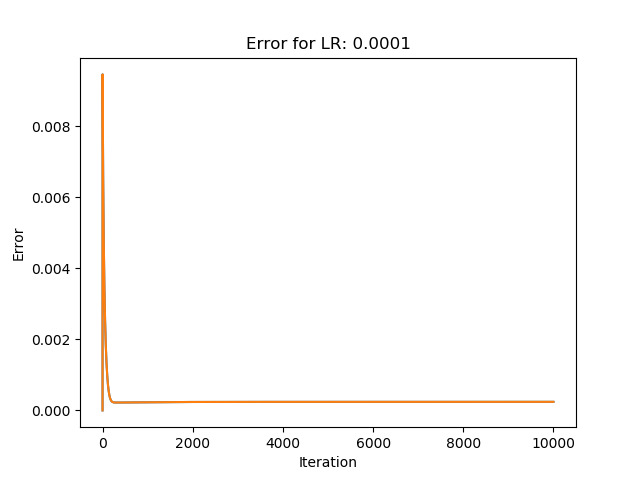
\includegraphics[width=12cm, scale=0.5]{00001.jpg}
	\caption{Best Learning Rate was 0.0001}
	\label{fig:LR_00001}
\end{figure}


%----------------------------------------------

\begin{question}{Gradient Descent Variants}{5}
Throughout this class we have seen that gradient descent is one of the most used optimization techniques in Machine Learning. This question asks you to deepen the topic by conducting some research by yourself.

\textbf{1)} There are several variants of gradient descent, namely \emph{batch, stochastic} and \emph{mini-batch}. Each variant differs in how much data we use to compute the gradient of the objective function. 
Discuss the differences among them, pointing out pros and cons of each one.

\textbf{2)} Many gradient descent optimization algorithms use the so-called \emph{momentum} to improve convergence. What is it? Is it always useful?

\begin{answer}



\textbf{Batch gradient descent} in machine Learning calculates the gradient using the whole dataset. For this the computer needs to have the whole dataset in memory, which is not always doable. Because of that, its also very time consuming. It converts against the global Minimum of konvex functions and local Minimums of non konvex functions.

\textbf{Stochastic gradient descent} calculates the gradient for a single traingingexample. Because of this stochastic gradient descent learns a lot faster than batch gradient descent, however its variance is very high, resulting in highly fluctuating costfunction.


\textbf{Mini-batch gradient descent} can be seen as an combination between stocahstic gradient descent and batch gradient descent, using mini-batches containing $n$ training examples. This results in reduced variance and more stable conversion rate. When mini-batch gradient descent is calculated on gpus, it is possible to reduce the workload by using matrix operations.


\textbf{Momentum} is often used to help the gradient descent algorithm to find the global Minimum. 

Without Momentum there is a high possibility, that GD starts oscillating around a local minimum. In order to reach the global Minimum, this local one needs to be "jumped over". This can be interpeted as a physical impulsive giving a downhill rolling sphere an impuls of energy, to help it overcome obstacles. This "impuls" is usually calculated by looking at the last gradient and adding a part of it to the current gradient. This means, that if the last update to our parameters was big, we guess that the next one will be big, too.
\end{answer}

\begin{figure}[h!]
	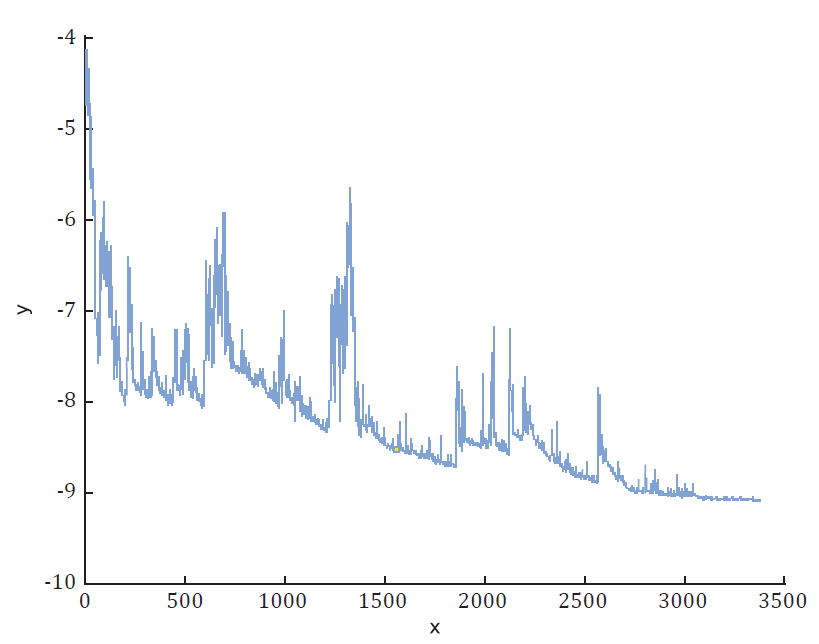
\includegraphics[width=12cm, scale=0.5]{SGD.png}
	\caption{Example for fluctuating cost function for a Neural Network when using SGD [Source: Me]}
	\label{fig:SGD_cost_function}
\end{figure}
\begin{figure}[h!]
	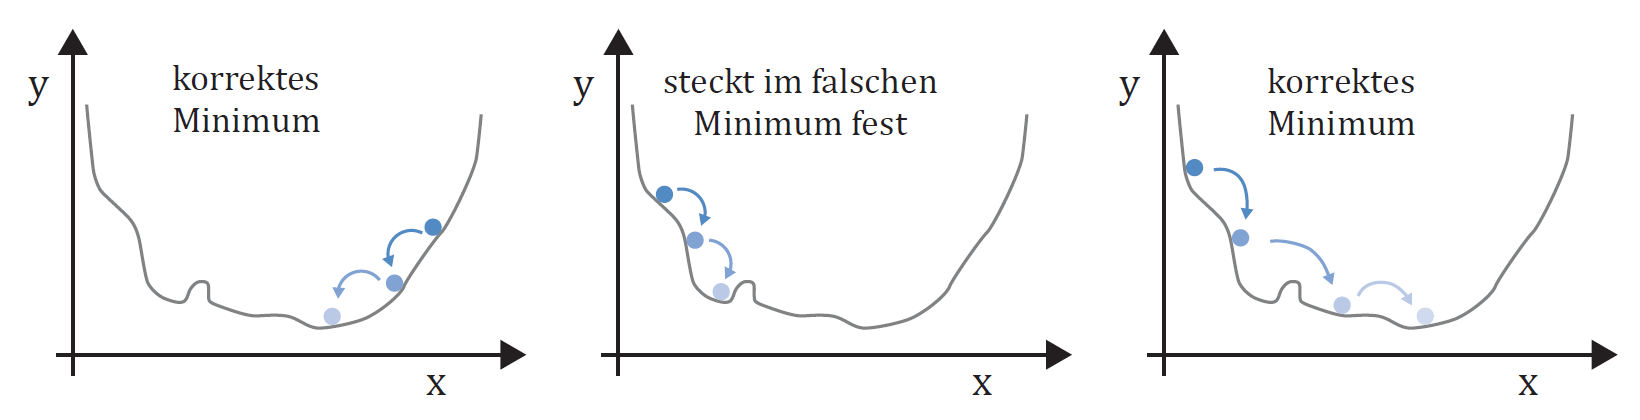
\includegraphics[width=\linewidth, scale=0.5]{momentum.png}
	\caption{Physically interpretation of Momentum [Source: Me]}
	\label{fig:Momentum}
\end{figure}


\end{question}
%----------------------------------------------

\begin{question}[bonus]{Natural Gradient}{10}
Let $\theta \in \mathbb{R}^n$ be a parameter vector
and $J \colon \mathbb{R}^n \to \mathbb{R}$ a cost function.
The negative gradient $-\nabla J(\theta)$ is sometimes called
the \emph{steepest descent direction}. But is it really?
To be able to claim that it is \emph{the} steepest descent direction,
we should compare it to other descent directions
and pinpoint what is so unique about the negative gradient direction.

\textbf{Covariant gradient.}
A fair way to compare descent directions is to make
a small step of fixed length, say $\varepsilon$,
in every direction~$\Delta \theta$ and check
which direction leads to the greatest decrease in $J(\theta)$.
Since we assume that the step size is small, we can evaluate
the decrease in $J(\theta)$ using its first-order Taylor approximation
\begin{equation*}
  J(\theta + \Delta \theta) - J(\theta) \approx
  \nabla J(\theta)^T \Delta \theta.
\end{equation*}
To make precise what we mean by \textit{small} step size,
we need to introduce a norm (or a distance)
in the space of parameters $\theta$.
A good choice, that among other advantages captures the intuition
that some parameters may influence the objective function more
than others,
is the generic quadratic norm
\begin{equation*}
  \norm{\Delta \theta}^2 =
  \frac{1}{2}\Delta \theta^T F(\theta) \Delta \theta
\end{equation*}
with a positive-definite matrix $F(\theta)$;
note that in general $F$ may depend on $\theta$.

\textbf{1)} Find the direction $\Delta \theta$ that yields
the largest decrease in the linear approximation of $J(\theta)$
for a fixed step size~$\varepsilon$.
Does this direction coincide with $-\nabla J(\theta)$?
The direction that you found is known as the
negative covariant gradient direction.

\textbf{Natural gradient.}
In statistical models, parameter vector $\theta$ often
contains parameters of a probability density function $p(x; \theta)$
(for example, mean and covariance of a Gaussian density);
thus, the cost function $J$ depends on~$\theta$ indirectly
through $p(x; \theta)$.
This two-level structure gives a strong hint to what matrix $F$
to pick for measuring the distance in the parameter space
in the most \textit{natural} way.
Namely, one can carry over the notion of `distance' between
probability distributions $p(x; \theta + \Delta \theta)$
and $p(x; \theta)$ (which is known from information theory
to be well captured by the Kullback-Leibler divergence)
to the distance between the corresponding parameter vectors
$\theta + \Delta \theta$ and $\theta$.

\textbf{2)} Obtain the quadratic Taylor approximation
of the KL divergence
from $p(x; \theta)$ to $p(x; \theta + \Delta \theta)$ in the form
\begin{equation*}
  KL(p(x; \theta + \Delta \theta) || p(x; \theta)) \approx
  \frac{1}{2}\Delta \theta^T F(\theta) \Delta \theta.
\end{equation*}
Covariant gradient with the matrix $F(\theta)$ that you found
is known as the natural gradient.

\begin{answer}\end{answer}

\end{question}



%----------------------------------------------

\end{questions}


\end{document}
